\pagebreak
\section{Analysis and Results: How do Machine Learning Methods Perform at Forecasting Inflation?} \label{sec:analysis}

\subsection{Overall Results}


\begin{figure}[H]
    \centering
    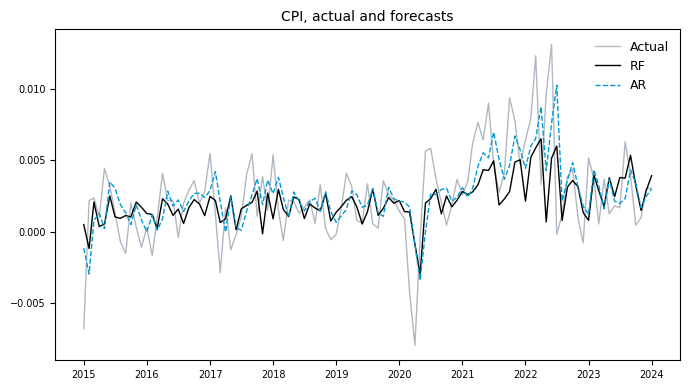
\includegraphics[width=1\linewidth]{figures/forecasts.png}
    \vspace{-30pt}
    \caption{CPI change, actual and forecasts, 1960-2024.}
    \label{fig:cpi} 
\end{figure}


\subsection{Model-specific Discussion}

\subsubsection{Lasso}

Bad because maybe you can't improve on normal factor models \autocite{GouletCoulombe2022HowForecasting}

Bad also maybe because no polynomial features. Size of model also meant I had to give it wider paramters to converge.

Tried ot do a polynomial model to increase accuracy (list the strategies) and it was still too large. 